\documentclass[border=10pt]{standalone}
\usepackage{tikz}
\usetikzlibrary{
  calc
}
\usepackage{pgfplots}

\pgfplotsset{
  colormap={spectrum}{
    color(0.00000000000000bp)=(violet);
    color(8.33333333333333bp)=(blue);
    color(16.66666666666670bp)=(cyan);
    color(25.00000000000000bp)=(green);
    color(33.33333333333330bp)=(yellow);
    color(41.66666666666670bp)=(orange);
    color(50.00000000000000bp)=(red)
  }
}
\begin{document}


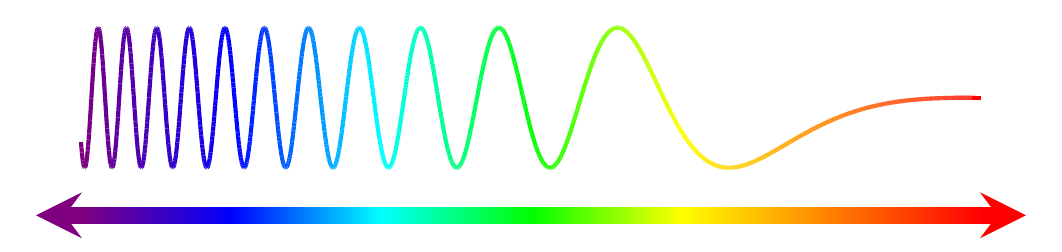
\begin{tikzpicture}
  % define the unit
  [x=1in, y=0.35in]

  \begin{axis}
    [
      % tell pgfplot to use the same unit as tikz
      x=1in, y=0.35in,
      % the size of pgfplot
      % width=5in, height=1in,
      % set the domain of the function
      domain=-4.5:0,
      % only show the domain
      xmin=-4.5, xmax=0,
      % ymin=-1.8,
      % do not show the spines of the axes
      axis lines=none,
      % define the colormap, bluered inverted
      colormap name=spectrum,
      % if you use 'rel axis cs', add this to show contents out of the axis
      clip=false,
      % colorbar settings
      colorbar horizontal,
      colorbar style = {
        at = {(0, -0.20)},
        height=6pt,
        anchor=west,
        axis lines=none,
        % ticks=none,
      }
    ]
    \addplot[
      mesh, point meta=x,
      % number of points
      samples=2000,
      line width=1.5pt,
    ] {
      % the function of the spectrum
      sin(45*x^3)
    };

    % add arrows to both ends of the colorbar
    \draw[
      ->, >=stealth,
      line width=6pt, anchor=east, color=violet
    ] (rel axis cs: 0, -0.20) -- (rel axis cs: -0.05, -0.20);
    \draw[
    ->, >=stealth,
    line width=6pt, anchor=west, color=red
    ] (rel axis cs: 1, -0.20) -- (rel axis cs: 1.05, -0.20);
  \end{axis}
\end{tikzpicture}

\end{document}
